
%Define refactoring referring mainly to Brown et al. (1998) and Fowler (2000). 
%Explain the importance and benefits of refactoring referring to at least Khomh et al. (2009), Cusumano et al. (1997), Cusumano et al. (1997)

%In addition to the references mentioned in the sub-sections, take a look at the following papers:
%\begin{itemize}
%\item Yamashita and Leon (2012)
%\item Yamashita and Leon (2013)
%\item Mäntylä (2009)
%\item Arcoverde et al. (2011)
%\item Mäntylä (2005)
%\item Mäntylä and Lassenius (2006)
%\end{itemize}

The term software refactoring was introduced for the first time by William F. Opdyke in his Ph.D. dissertation \cite{opdykeRefactoring}. It became more practical and commonly used after the publication of the book Refactoring: Improve the Design of Existing Code, which is written by Martin Fowler in the year 1999 \cite{fowlerRefactor}. 

Software refactoring is a form of code modification, used to improve the software structure in support of subsequent extension and long-term maintanence, in most cases having the goal to transform code without impacting correctness \cite{brownAntiPatterns}. The basic principle in refactoring process is reorganizing classes, variables and methods across the class hierarchy to facilitate future adaptations and extensions, so that the source code can have better structure, readability and understandability \cite{abebeLiterature}. 

%Refactoring, the act of modifying software structure without changing its observable behaviour, 
Refactoring is important in order to maintain and improve code evolvability \cite{mantylaDrivers}. While the primary goal is to produce good quality code from the beginning, refactoring became a key practice of agile development, and applied as a building block to compensate the lack of upfront design \cite{mantylaDrivers}.

%Refactoring is the process of making small code level changes to improve its internal structure. The cumulative effect of these small changes can radically improve software design \cite{fowlerRefactor}. With refactoring the software design is formed continuously during development rather then up front. 

Refactoring is also performed to make the software more readable. Refactoring does not change the observable behavior of the software. Software still carries out the same function that it did before. Any user, whether an end user or another programmer, can not tell that things have changed \cite{fowlerRefactor}.  

Refactoring can be used as a mean to improve the maintainability of the code by making the code conform to coding standards, minimizing redundancies, improving language proficiency, improving safety and portability, and raising the quality of the documentation \cite{siyInspection}.

%Then why refactor? Refactoring improves the design of the software, makes software easier to understand, helps to find bugs and to program faster.

According to a survey on software refactoring \cite{mensSurvey}, the refactoring process consists of a number of distinct activities:

\begin{enumerate}
\item Identify where the software should be refactored.
\item Determine which refactoring(s) should be applied to the identified places.
\item Guarantee that the applied refactoring preserves behavior.
\item Apply the refactoring.
\item Assess the effect of the refactoring on quality characteristics of the software (e.g., complexity, understandability, maintainability) or the process (e.g., productivity, cost, effort).
\item Maintain the consistency between the refactored program code and other software artifacts (such as documentation, design documents, requirements specifications, tests, etc.).
\end{enumerate}

This study mainly discusses the first two activities; \textit{identifying where the software should be refactored} (drivers) and \textit{determining which refactoring(s) should be applied} (solutions). Accordingly, this section presents refactoring reasons addressed in the literature, namely code smells and development anti-patters. Proposed refactoring solution is also described under each refactoring reason.

\subsection{Refactoring reasons}  
%Admit the basis of the presented taxonomy comes from Fowler (2000) but it is inspired (or taken from) Mäntylä et al. (2003). 
%Attempt to discuss and improve the taxonomy with at least Brown et al. (1998), Mäntylä and Lassenius (2006), Yamashita et al. (2013)

Identifying where to refactor can be challenging and it is difficult to locate existing problematic parts in code known as code smells and anti-patterns. However, once these bad designs are detected, they can serve as significant drivers for software refactoring decisions. 

The objective of this literature study is to identify the most significant refactoring reasons found in the literature and grasp an understanding on how they relate to our empirical findings.The reasons are presented in two categories; code smells \cite{fowlerRefactor}, development level anti-patterns \cite{brownAntiPatterns}. 

\subsubsection{Code smells}
"Code smells" or "bad smells" are structures in code that suggest the possibility of software refactoring \cite{fowlerRefactor}. Code smell do not indicate how to solve the problematic code, but it narrows down the numbers of potential refactoring solutions that can be applied. Fowler provides a list of code smells with their corresponding refactoring solutions to make the refactoring decision easier \cite{fowlerRefactor}.

Fowler identifies code smells that primarily appear in object-oriented design. As refactoring solutions they recommend object-oriented design patterns to satisfy concepts such as; interacting objects, information hiding, inheritance, interfaces, and polymorphism. Therefore, code smells can be derived based on poorly used, over-used, or misused object-oriented design principles. 

As a supporting work, Mäntylä et al. introduces a taxonomy based on Fowler's 22 smells to make the smells more understandable and to disclose the relationships among them \cite{mantylaTaxonomy}. Owing to their classification, this section specifies the 22 smells in seven categories; bloaters, object-orientation abusers, change preventers, dispensables, encapsulators, couplers, and others. 

\subsubsection*{Bloaters}
Bloaters represent something in the code that has grown so large that it cannot be effectively handled \cite{mantylaTaxonomy}. This category include code smells including, long method, large class, primitive obsession, long parameter list, and data clumps.

\textit{\textbf{Long method -}} the software that lives best and longest are those with short methods \cite{fowlerRefactor}. The longer a method body is, the more difficult it is to understand. It is usually more vulnerable to possible bugs due to having more corner cases to cover.

Earlier programming languages and development environments have deterred people from small methods. These Languages introduced overhead in subroutine calls and available tools made it difficult to switch context between routines and subroutines. However, modern languages and integrated development environments (\gls{IDE}), have overcome these shortages. The net effect is that developers can be more aggressive when decomposing methods to improve understandability, robustness and modularity.  

The propesed refactored solutions \cite{fowlerRefactor} on long methods include:

\begin{itemize}
\item Replace comments with methods to reduce the semantic distance between what methods does and how it does it.
\item Shorten methods by extracting code parts that seems to go nicely together into their own subroutines.
\item To overcome method extraction issues when when there are lots of temp variables, conditionals and loops, decompose them into utility methods 
\item To overcome method extraction issues when a method has a long parameter list, introduce parameter objects.  
\item If a method still can not be decomposed easily, turn the method into its own object so that all the local variables become fields of it's own and then decompose the method into other methods on the same object. 
\end{itemize}

\textit{\textbf{Large class -}} reveals to much responsibility. When a class is trying to do too much, it often shows up too many instance variables. This brings a lot of duplicated code into existence. A large class is also commonly exposed to changes for different reasons. This introduces extra complexity when software changes are required.

Two refactoring solutions are suggested for a class with too much code -- a prime breeding ground for duplicated code, chaos, and death \cite{fowlerRefactor}. 

\begin{itemize}
\item Extract class and split the responsibility. 
\item Extract subclass for a subset of features. If a class has features that are used only in some instances, extract that subset into a subclass.
\end{itemize}

\textit{\textbf{Primitive obsession -}} most programming languages have two data types -- primitives and objects. Primitive type is a simple type holding a single value to represent a single data item. Objects on the other hand, allows to structure data items into meaningful groups. If a data item needs to be represented rather comprehensively, by using primitives one needs to extend the owning class with methods to satisfy the requirements. This can quickly result in code smells of duplication and feature envy.

In order to represent comprehensive data items without introducing code smells several refactoring solutions have introduced \cite{fowlerRefactor}:

\begin{itemize}
\item Replace data value with object. Turn the data item into an object once it requires additional data or behaviour.
\item If the data value is a type code and does not affect class behaviour, replace it with class. By wrapping numeric type codes and enumerations into a class and providing static factory methods for handling them, readability of the code can be improved and potential bugs can be prevented.  
\item If the type code is affecting class behaviour, replace type code with subclass. Form an inheritance structure having a subclass for each type code. Following this, replace conditionals that depend on the type codes with polymorphism
\end{itemize}

\textit{\textbf{Long parameter list -}} having method parameters is an alternative to having global variables. However, this is only true in our early programming days. However in an object-oriented context, instead of using a long parameter list or declaring global variables, a method can request data from other objects. Thus, instead of passing everything a method needs, it is enough to pass parameters so that the method can retrieve relevant data. 

Refactoring solutions are introduced for long parameter lists \cite{fowlerRefactor} that reduces the likelihood of having methods that are inconsistent, difficult to use, understand, maintain and change:

\begin{itemize}
\item Replace parameter with method. If a method can get a value that is passed in as parameter by another means, it should \cite{fowlerRefactor}. If a method parameter is formed of an expression, the parameter can be removed by extracting the expression intro a subroutine and calling it directly from the method. 
\item Use preserve whole object. If several values of an object is passed as parameters into a method, instead, the whole object can be passed as a parameter or an appropriate method of the whole object can be invoked that returns required values.
\item Introduce parameter objects based on group of data that naturally go together.Data clumps which are typically passed together as parameters, can be replaced with objects that wraps them. 
\end{itemize}

\textit{\textbf{Data clumps -}} are one of the causes of long parameter lists, long methods, and large classes. Until they are extracted into a class, data items that naturally go together float within code and cause duplication, inconsistency, maintainability and readability issues.

This code smell can be resolved by using class extraction to split responsibility, previously explained on \textit{large class} code smell. Data clumps can be further served as parameter objects or, preserved as whole objects. Both refactoring solution was elaborated on \textit{long parameter list} code smell.

\subsubsection*{Object-orientation abusers}
This category of smells is related to cases where the solution does not fully exploit the possibilities of object-oriented design \cite{mantylaTaxonomy}. Switch statements, temporary field, refused bequest, alternative classes with different interfaces, and parallel inheritance hierarchies are considered in the object-orientation abusers category. 

\textit{\textbf{Switch statements -}} result in duplicated code and a significant maintainability issue when code is subject to change. It causes duplication since the same statement typically exists in multiple places. In conjunction with duplication, it significantly prevents change. If a switch statement needs an additional clause, the change needs to be applied in all places where the statement is used.

The proposed refactoring solutions \cite{fowlerRefactor} indicate using the object-oriented notion of polymorphism.

\begin{itemize}
\item If a switch statement occur on a type code, similar to the refactoring solutions proposed on the \textit{primitive obsession} code smell, an inheritance structure can be formed having a subclass for each type code. Following this, switch statements can be replaced with polymorphism.
\item If there are only few cases which makes using polymorphism an overkill, add an explicit method for each conditional case in the switch statement.
\end{itemize}

\textit{\textbf{Temporary field -}} smell occurs in the case where a class variable is only set and used in certain cases. For instance, a temporary variable could be defined in the class scope, whereas it should only be defined a method scope. This type of smell make it difficult to understand the duty of the temporary variable. 

In order to resolve this type of code smell, temporary fields and the methods that require them can be extracted into a new class \cite{fowlerRefactor}. The new method object can then be used by the original class. 

\textit{\textbf{Refused bequest -}} smell is a sign of an inappropriate inheritance hierarchy. Subclasses get to inherit the methods and data of their parents \cite{fowlerRefactor}. This smell occurs when there is clash between what subclass expects to reuse and what it inherits from the parent class.

There are two refactoring solutions proposed to resolve the conflict on the inheritance hierarchy:

\begin{itemize}
\item Heading towards having an abstract superclass by pushing down fields and methods to subclasses.
\item Removing the inheritance hierarchy and replacing inheritance with delegation. This solution can be used in the case where the subclass is refusing the superclass interface and causing the inheritance hierarchy to be useless. Instead, the superclass can be declared as a class variable and used appropriately. 
\end{itemize}

\textit{\textbf{Alternative classes with different interfaces -}} smell is a sign of not using inheritance properly on closely related classes. These classes contain similar features which can be considered as duplicate code and a preventer for change.

As a refactoring solution the commonalities can be extracted into a superclass. Consequently, the alternative classes can be incorporated in a inheritance hierarchy.

\textit{\textbf{Parallel inheritance hierarchies -}} smell needs to be fixed by using a proper inheritance hierarchy. Tightly coupled classes result in tightly coupled inheritance hierarchies. This results as a special case of the \textit{shotgun surgery} code smell having duplicated code\cite{fowlerRefactor}. 

The proposed refactoring solution to eliminate duplication is to make sure that instances of one hierarchy refer to instances of the other. This means decoupling classes that have a parallel inheritance hierarchy. Achieving this requires moving methods and fields from one class to the other and using only references. As a result the inheritance hierarchy on the referring class will disappear \cite{fowlerRefactor}.  

\subsubsection*{Change preventers}
Change preventer code smells imply code structures that considerably hinder the modification if the software.  \cite{mantylaTaxonomy}. Ideally according to \cite{fowlerRefactor}, there is a one-to-one link between common changes and classes. This category contains divergent change and shotgun surgery code smells:

\textit{\textbf{Divergent change -}} is one type of smell that causes difficult to modify code. It occurs when a class acts feature envy containing various responsibility, as a result being exposed to change in different ways for different reasons. Any change to handle a variation should change a single class, and all the typing in the new class should express the variation \cite{fowlerRefactor}.

As a refactoring solution, one must identify all changing blocks for a particular cause and extract them into a new class. 
 
\textit{\textbf{Shotgun surgery -}} in the other code smell type that causes difficult to modify code. It occurs when a change has an effect on multiple locations. It is considerably difficult to modify certain part of a software, if it requires multiple changes in multiple classes.

Proposed refactoring solution suggests moving methods/fields to another class and access them via reference. Thus, code blocks affected by a particular change is put into a single class. 

\subsubsection*{Dispensables}
This type of code smells indicate existing unnecessary peaces in the code. This could be related to having lazy, redundant, or dead peaces in the code. Interestingly, Fowler \cite{fowlerRefactor} do not present a smell for dead code. Dead code is code that is left behind due to legacy reasons, evolved software, changed requirements, or refactoring. Dead code hinders code comprehension and makes current code structure less obvious \cite{mantylaTaxonomy}.

Dispensable code smells include, lazy class, data class, duplicated code, and speculative generality.

\textit{\textbf{Lazy class -}} is a class that is not doing enough work and suitable to be eliminated with a short effort. 

There are two refactoring solutions proposed to eliminate a lazy class:

\begin{itemize}
\item Code in a nearly useless class can be moved to another class. 
\item In a inheritance hierarchy, if a subclass is not adding any value, the hierarchy can be collapsed. The methods and fields in the subclass can be pulled up to the parent class.
\end{itemize}
 
\textit{\textbf{Data class -}} is a simple class that only have data fields and getter/setter methods for the fields. Similar to a lazy class, it does not have enough responsibility. Yet in this case, it is more suitable to embrace extended functionality. 

There are several building blocks to extend the responsibility of a data class:

\begin{itemize}
\item First of all, encapsulation should be applied to its publicly available variables.
\item Setter methods should be removed for variables that should not be modified.
\item The behaviour of the outsider methods that invoke the getter and setter methods of the data class can be moved to the data class.
\item Finally, encapsulation can be applied to its methods that are not used by other classes.
\end{itemize}

\textit{\textbf{Duplicated code -}} smell indicates having the same code structure in multiple places. When a modification is required in such a code structure, the same change need to be applied in multiple locations.

The proposed refactoring solution recommends unifying recurring code in a method. This can be achieved in steps; 
\begin{enumerate}
\item Extract duplicated code as a separate method.
\item Decide where the new method should belong.
\item Ensure that only this methods is called from all locations that seek the functionality.
\item Remove its duplicates.
\end{enumerate}

\textit{\textbf{Speculative generality -}} smell occurs when unnecessary ability is introduced to the code for the sake of speculative reasoning. This often results in a code with unused parts that is difficult to understand and maintain. 

The refactoring solutions used to eliminate speculative generality include:

\begin{itemize}
\item If abstract classes are used that does not add any value, inheritance hierarchy can be collapsed.
\item Unnecessary delegation can be resolved by moving the functionality indoors.
\item Unused method parameters should be removed.
\item Methods having difficult to understand abstract names should be renamed.
\item Identify methods/classes that are only used in test cases. Remove them in case they are not supportive for test cases that exercise legitimate functionality. 
\end{itemize}

\subsubsection*{Encapsulators}
Encapsulation means hiding internal details from other classes. \cite{fowlerRefactor}. Code smells in this category reveal issues on the way objects, data, or operations are accessed. The smells in this category are message chains and middle man. 

\textit{\textbf{Message chain -}} smell usually indicates a coupling problem. When there is a chain of tightly coupled classes, modifying one requires changes on others.

Refactoring solution proposes hiding delegates using the following steps:

\begin{itemize}
\item Add a simple delegate method on the middle man. 
\item Adjust the caller class to call the delegate method on the middle man.
\item Remove direct access to the delegate object on the middle man.
\end{itemize}. 
 
\textit{\textbf{Middle man -}} is a result of applying excessive amount of encapsulation and delegation. In this case, a class can become a middle man.

Different refactoring solutions can be applied in this case, depending on the condition of the class:

\begin{itemize}
\item If the class is nothing but a middle man, it can be removed, and the caller classes may start accessing its delegates directly
\item If only a few method is used as delegates, move those methods to the caller class.
\item If you have many simple delegations for the entire interface and if there is additional behaviour that stops your from removing the middle man, replace delegation with inheritance and make the delegating class (middle man) a subclass of the delegate. This will allow to extend delegate behaviour without any chaining.
\end{itemize} 

\subsubsection*{Couplers}
High coupling is against object-oriented design principles. It dramatically reduces the ability to modify and reuse software components. Code smells in this category are highly related to object-orientation abuser smells. This category includes, feature envy and inappropriate intimacy smells.

\textit{\textbf{Feature envy -}} smell means a case where one method have a lot of responsibility and more interested in other classes then the owning class. This smell clearly indicates that such a method belongs elsewhere. 

Depending on the method condition, several refactoring solutions can be applied:

\begin{itemize}
\item If it is obvious that the method belongs to a particular class, it can be moved. The method should go together with the data that it uses and the idea is to put things together that change together. This rule of thumb can be used in deciding a correct location for such a method.
\item In case only one part of the method suffers from envy, that part can be extracted and moved as a new method to the relevant class.
\end{itemize}
 
\textit{\textbf{Inappropriate intimacy -}} means that two classes are tightly coupled with each other \cite{mantylaTaxonomy}. In such a case, following refactoring solutions can serve several approaches:

\begin{itemize}
\item Moving over-intimately used methods or fields to the correct class and improve decoupling.
\item Change bidirectional associations to unidirectional. Bidirectional associations introduce added complexity of maintaining the two-way links and ensuring that objects are properly created and removed \cite{fowlerRefactor}. Additionally, they are usually not perceived as natural by developers, so they often are a source of errors \cite{fowlerRefactor}.
\item Hide delegate to reduce intimacy and introduce a middle man class for accessing delegates.
\item If inheritance is causing inappropriate intimacy, replace it with delegation. At the subclass, create a field for the parent class, adjust methods to delegate to the parent class, and remove the inheritance hierarchy.
\end{itemize}

\subsubsection*{Others}
This category contains code smells that do not fit into any of the above categories. It covers incomplete library class and comments.

\textit{\textbf{Incomplete library class -}} code smell occurs in case a library is in a bad form and impossible to modify. Under this circumstances, as a refactoring solution, one can introduce foreign methods or classes as a local extension. This way, they could be further refactored and modified according to needs. 
 
\textit{\textbf{Comments -}} in code can be an indication of a bad smell nearby. The best practice is to go through code comments, identify the bad smells nearby and refactor. Refactoring nearby code smell can transform code comments to be unnecessary.

Possible refactoring solutions include:

\begin{itemize}
\item If a block of code requires comment, extract that block into a new method and assign a descriptive name.
\item If a method body is hard to understand and requires comment, rename the method to be more explanatory.
\item if a block of code relies on an assumption, make that assumption explicit by introducing an assertion.
\end{itemize}

On the other hand, comments can be used as a refactoring solution themselves. It can be useful to add comments to describe why something was implemented in such a way, or how it can be improved. 

Martin extended the work of Beck and Fowler with an elaboration on a set of design principles and new smells that were advocated by the Agile community \cite{martinAgile}.

\subsubsection{Development anti-patterns}
An anti-pattern is defined by Brown et al. \cite{brownAntiPatterns} as a commonly occurring solution that will always generate negative consequences when it is applied to a recurring problem. In their book, Brown et al. describes anti-patterns in three levels including, development, architecture, and project management. This section only descrives development level anti-patterns, since we are only interested in code level refactoring decisions, 

Development anti-patters are conjectured in the literature to make systems harder to maintain. Moreover, code smells presented in the previous section can be seen as being symptoms of these anti-patterns. Even though they overlap, there are anti-patterns which are not referred in code smells.  

\subsubsection*{The blob}
The blob is found in designs where on class controls all the processing while others act like simple data classes. A blob is an outcome of a procedural design even though it may be represented using object notations and implemented in object-oriented languages. Therefore, as in procedural design, the blob contains the majority of processes while the other objects contain only data. 

Several code smell can be a symptom of the blob anti-pattern. \textit{Large class} smell may contain the blob anti-pattern if it controls all the processes. This will leave the rest of the classes to act as a \textit{Data class} or \textit{lazy class}. This anti-pattern can also be a sign of a \textit{Large class} having a lot of \textit{Feature envy} methods, while other \textit{Data classes} having \textit{Inappropriate intimacy}. 

\textit{Divergent change} code smell is another symptom of this anti-pattern. A blob class controlling most of the processes, is exposed most to different changes for different reasons.

The solution includes refactoring the design to distribute responsibilities more uniformly and isolating the effect of changes. Detailed refactoring techniques can be found under related code smells. 

\begin{table}[ht!]
\centering
\caption{The blob anti-pattern view}
\label{table:blob}
    \begin{tabular}{ p{5cm} p{9cm} }
     \hline
     \textbf{Related smell groups}   &Bloaters, Change preventers, Dispensables, Couplers\\ 
     \hline
     \textbf{Related code smells}   &Large class, Divergent change, Data class, Lazy class, Inappropriate intimacy\\ 
     \hline
     \textbf{Refactoring solution}  &Applying proper decomposition and distributing responsibilities more uniformly to other classes\\ 
     \hline
    \end{tabular}
\end{table}

\subsubsection*{Lava flow}
Lava flow anti-pattern imply dead code and forgotten design information left as legacy in an evolving software. As a consequence, code that are redundant, commented out, or not understood by anyone is left behind in the software, Unless these symptoms are cleaned, the software is difficult to extend, maintain and understand. 

Lava flow is clearly related to the \textit{Dispensables} code smell group. However, Fowler \cite{fowlerRefactor} does not mention dead code as a code smell. 

The refactored solution includes a configuration management process that eliminates dead code and refactors software design toward increasing quality. This configuration management process can be strictly executed as part of the architectural configuration management, however, in agile development process it can be informal and tight to intensive face-to-face communication, pair reviews, and shared code ownership. 

\begin{table}[ht!]
\centering
\caption{Lava flow anti-pattern view}
\label{table:LavaFlow}
    \begin{tabular}{ p{5cm} p{9cm} }
     \hline
     \textbf{Related smell group}   &Dispensables\\ 
     \hline
     \textbf{Refactoring solutions}  &In architecture-centric development processes, introducing a configuration management process to eliminate dead code and refactor software design in architecture-centric development processes.\\ 
     &In agile development processes, relying on intensive face-to-face communication, pair reviews, and shared code ownership to eliminate redundancies \\
     \hline
    \end{tabular}
\end{table}

\subsubsection*{Functional decomposition}
Functional decomposition is a direct match with the \textit{Object-orientation abusers} code smell group. It refers to the misuse of object-orientation and resulting with code that resembles a structural language in class structure.

\begin{table}[ht!]
\centering
\caption{Functional decomposition anti-pattern view}
\label{table:functionalDecomposition}
    \begin{tabular}{ p{5cm} p{9cm} }
     \hline
     \textbf{Related smell group}   &Object-orientation abusers\\ 
     \hline
     \textbf{Refactoring solutions}  &Reengineering object-orientation\\
     \hline
    \end{tabular}
\end{table}


\subsubsection*{Poltergeists}
Poltergeists are classes with very limited roles and effective life cycles. This anti-pattern, depending on its condition, is a direct match to the \textit{Data class} or \textit{Lazy class} code smell.

\begin{table}[ht!]
\centering
\caption{Poltergeists anti-pattern view}
\label{table:Poltergeists}
    \begin{tabular}{ p{5cm} p{9cm} }
     \hline
     \textbf{Related smell groups}  &Dispensables\\
     \hline
     \textbf{Related code smells}  &Data class and Lazy class\\
     \hline
     \textbf{Refactoring solutions}  &Reallocating responsibilities to longer-lived objects that help mature data classes or eliminate lazy classes, as a result remove poltergeists\\
     \hline
    \end{tabular}
\end{table}

\subsubsection*{Golden hammer}
This anti-pattern appears as one particular programming solution is applied in a diverse range of problems, even though there might be better solutions. The reason could be taking less risk, or neglecting to learn new approaches. As a result, this anti-pattern may introduce inferior performance, scalability, and so on when compared to other available solutions. 

None of Fowler's code smells can be seen as a symptom of this anti-pattern.

\begin{table}[ht!]
\centering
\caption{Golden hammer anti-pattern view}
\label{table:GoldenHammer}
    \begin{tabular}{ p{5cm} p{9cm} }
     \hline
     \textbf{Refactoring solutions}  &There are no direct code level refactoring solutions, however, process level improvements include, managing knowledge transfer, taking more risk and responsibility, and developing competences\\
     \hline
    \end{tabular}
\end{table}

\subsubsection*{Spaghetti code}
Spaghetti code appears in a software which contains very less software structure. This anti-pattern is the most widely known design problem and, even though nonobject-oriented languages are more susceptible, it is also seen in the object-oriented context.

Spaghetti code may exist where there is a \textit{Large class}, a \textit{Long method}, or a \textit{Divergent change} code smell. It may also intro tight coupling, therefore, \textit{Couplers}, namely \textit{Feature envy} and \textit{Inappropriate intimacy} smells may easily exist. Additionally, most of class methods may be utilizing class or global variables instead of having parameters, which will cause a lot of \textit{Temporary field} smells. 

The examples can be extended, however, in summary, spaghetti code can expose the software to several group of code smells including, \textit{Object-orientation abusers, Change preventers} and \textit{couplers}.

\begin{table}[ht!]
\centering
\caption{Spaghetti code anti-pattern view}
\label{table:SpaghettiCode}
    \begin{tabular}{ p{5cm} p{9cm} }
     \hline
     \textbf{Related smell groups}  &Object-orientation abusers, Change preventers, Couplers\\
     \hline
     \textbf{Related code smells}  &Large class, Long method, Divergent change, Feature envy, Inappropriate intimacy, temporary field\\
     \hline
     \textbf{Refactoring solutions}  &This anti-pattern covers quite a lot of code smells and it is difficult to point specific refactoring suggestions. However, to discard spaghetti code, continuous refactoring and code cleanup should be practiced\\
     \hline
    \end{tabular}
\end{table}

\subsubsection*{Cut and paste programming}
Cut and paste programming is a clear blocker of software reuse and change. This anti-pattern is identified by the presence of duplicate segments of code spread through the software. Even though code duplication has a positive effect when to quickly make short-term modifications, in the long term it causes significant, reuseability and maintainability problems.

Cut and paste programming clearly matches with the \textit{Duplicated code} code smell, as well as it is highly related to the change preventer code smell \textit{Shotgun surgery}.

\begin{table}[ht!]
\centering
\caption{Cut and paste programming anti-pattern view}
\label{table:CutPaste}
    \begin{tabular}{ p{5cm} p{9cm} }
     \hline
     \textbf{Related smell groups}  &Change preventers and Dispensables\\
     \hline
     \textbf{Related code smells}  &Duplicated code and Shotgun surgery\\
     \hline
     \textbf{Refactoring solutions}  &Unifying duplicated code, ideally taking advantage of black-box reuse\\
     \hline
    \end{tabular}
\end{table}

\textit{Back-box reuse} enables reusing an external class or method without modifying it and without needing to know its implementation. It is an alternative to \textit{white-box reuse}, where developers take a class or method from elsewhere and modify it (i.e., via extending) according to specific needs. 

\subsubsection*{Other anti-patterns}
In addition to the described development anti-patterns, Brown \cite{brownAntiPatterns} explains several other "mini" anti-patterns including, \textit{Continuous obsolescence, Ambiguous viewpoint, Boat anchor, Dead end, Input Kludge, Walking through a minefield}, and \textit{Mushroom management}.
\begin{itemize}
\item \textit{Continuous obsolescence} anti-pattern is somewhat related to the \textit{Incomplete library class} code smell in which developers experience integration issues with external dependencies. 
\item \textit{Ambiguous viewpoint} anti-pattern is related to the misuse of architectural patterns such as Model-View-Controller(MVC) and object-orientation. 
\item A \textit{Boat anchor} is a direct match to the \textit{Speculative generality} code smell, which is a peace of software or hardware that serves no useful purpose. 
\item The \textit{Dead end} anti-pattern appears when there is an external component used within the software and that is no longer maintained and supported by the supplier. In this "dead end" scenario, similar steps can be taken as in the \textit{Incomplete library class} code smell. 
\item \textit{Input kludge} anti-pattern appears when ad hoc algorithms are employed for handling program's user input, in which case indicates the lack of precaution for problems that may occur due to program input. 
\item \textit{Walking through a minefield} anti-pattern indicates that, just because a software is released, it does not mean it is production ready. All software products contain defects and unless they are discovered through solid test coverage, bugs can appear on production and cause catastrophic problems. 
\item \textit{Mushroom management} anti-pattern may appear due to the isolation between developers and end users. If short feedback cycles are not performed, end user expectations can be easily misunderstood. 
\end{itemize}

\subsection{Developer perception towards refactoring}
Each refactoring decision has an underlying reasoning called as its refactoring rationale. Refactoring reasons can be found in literature as code smells and development anti-patterns. There are also other reasons which occasionally overlap and extend these smells and anti-patterns.

Surveys and empirical studies exist in literature, which provide quantitative results on refactoring rationales and how they are perceived by software professionals. Surveys present how these rationales are conceptually perceived, whereas, empirical studies reveal evidence on to which degree they are applied by professionals.

\subsubsection{Refactoring as a concept}

\textbf{>> Yamashita and Moonen, Do developers care about code smells: quantitative data out of their survey:}

In their exploratory study \cite{yamashitaDevelopers}, Yamashita and Moonen investigate developer perception of refactoring drivers (i.e. code smells and anti-patterns). Their survey conducted on 85 software professionals, reveals findings on developer knowledge about code smells and anti-patterns. As a result of their analysis, they present the extent of which refactoring drivers are a concern for software professionals and a ranking list of most popular code smells and anti-patterns. 

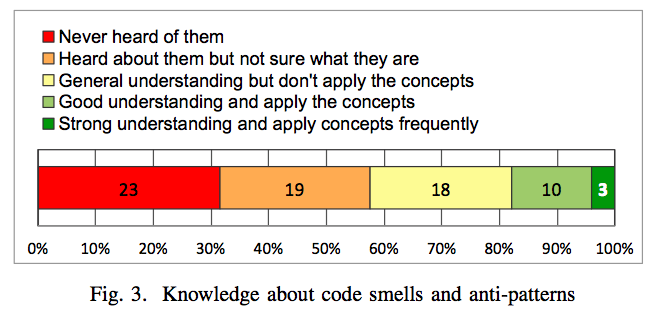
\includegraphics[width=\textwidth]{yamashita-smell-knowledge}

Even though the majority of their respondents were moderately concerned about code smells and anti-patterns, considerably large portion (32\%) of them did not know about refactoring drivers.

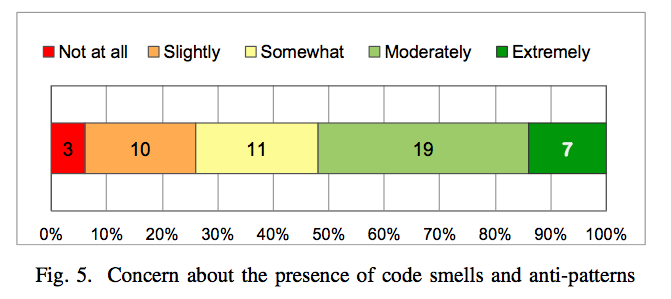
\includegraphics[width=\textwidth]{yamashita-smell-concern}

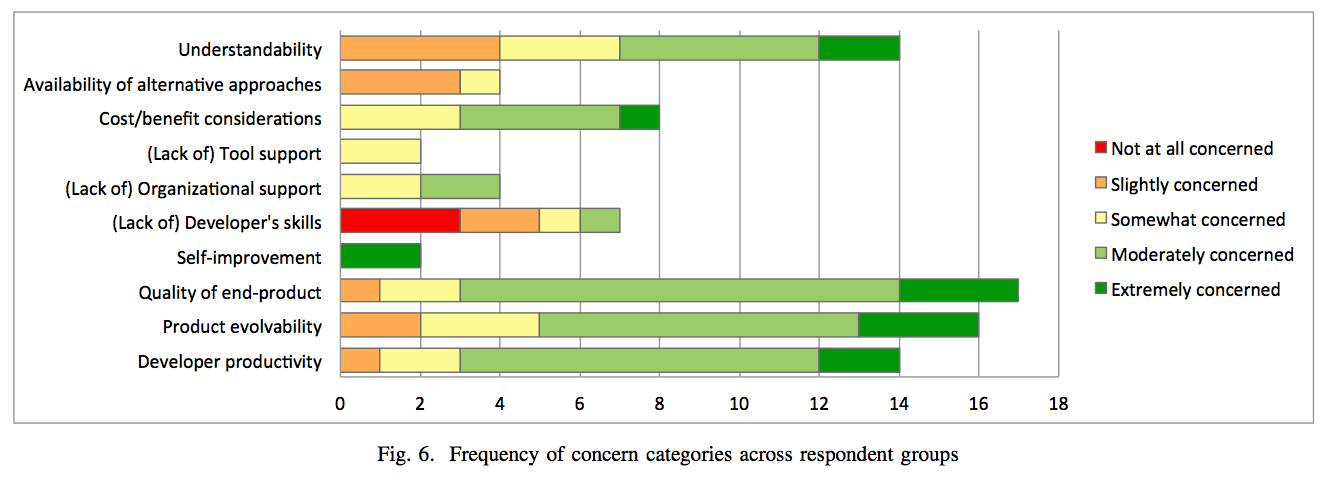
\includegraphics[width=\textwidth]{yamashita-smell-concern2}

Respondents who were moderate to extremely concerned gave as rationale reasons like product evolvability, end-product quality, and developer productivity. Respondents who were somewhat concerned about code smells indicated that it is often difficult to obtain organizational support, that they lacked adequate tools, and that they often need to make trade-offs between code quality and delivering a product on time.

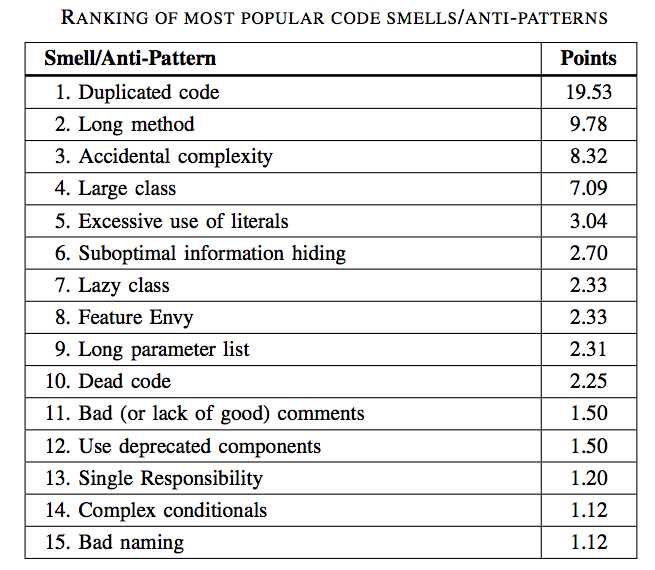
\includegraphics[width=\textwidth]{yamashita-smell-ranks}

Looking at individual smells and anti-patterns, duplicated code was mentioned most by the respondents, followed by drivers related to code size and complexity such as large class, long method, and the anti-pattern accidental complexity.

\textbf{>> Kim et al., A Field Study of Refactoring Challenges and Benefits: survey results}
In their survey of refactoring practices:

\subsubsection{Refactoring in practice}

\textbf{>> Siy and Votta, Does The Modern Code Inspection Have Value: empirical data out of their study:}

Siy and Votta have conducted an empirical study investigating the importance of code inspections and their findings indicate that it is a significant maintanence tool to identify so-called minor software defects that facilitate the evolution of code. They state that a significant part of inspection repair is spent fixing soft maintanence issues and fixing these issues lowers the cost of future changes to the code. We believe that their conclusions are exaclty inline with the benefits of refactoring. Refactoring can be seen as continuous code inspection and quality improvement. Moreover, refactoring is not merely an overhead of for the development process.

The main value of software inspection value has been seen as finding and fixing defects early in the development process in order to prevent the high cost of finding and fixing them later. However in the same way as refactoring, inspections also make the code easier to understand and change.

Siy and Votta's empirical results reveal that more than 90\% of soft maintenance issues were documentation and style recommendations. Specifecally, 47\% were documentation issues, 5\% were portability issues, 2\% were safety issues, and 46\% were style issues.

\textbf{>> Kim et al., A Field Study of Refactoring Challenges and Benefits: empirical data:}
In order to examine how the survey respondents’ perception matches reality in terms of refactoring and to investigate whether there are visible benefits of refactoring, Kim et al. decided to conduct interviews with a subset of the survey participants and to analyze the version history data.

Kim et al., in their quantitative analysis of historical data indicate that:
\begin{itemize}
\item Developers perceive that refactoring involves substantial cost and risks.
\item Refactoring change is likely to be more safe and reliable than regular change in a large system.
\item Refactored modules experienced higher reduction in the number of inter-module dependencies and post-release defects than other changed modules.
\end{itemize}

\textbf{>> Chidamber and Kemerer, A metrics suite for object oriented design: empirical data:}
Metric 1: Weighted Methods Per Class (WMC)
Metric 2: Depth of Inheritance Tree (DIT)
Metric3:Numberof Children(NOC)
Metric 4: Coupling between object classes (CBO)
Metric 5: Response For a Class (UFC)
Metric 6: Lack of Cohesion in Methods (LCOM)

Benefits of the metric suite which evaluates the condition of the 6 metrics:
\begin{itemize}
\item identify areas of the application that may require more rigorous testing and areas that are candidates for redesign. 
\item potential flaws and other leverage points in the design can be identified and dealt with earlier in the design- develop-test-maintenance cycle of an application. 
\item the added insight gained about trade-offs made by designers between conflicting requirements such as increased reuse (via more inheritance) and ease of testing (via a less complicated inheritance hierarchy).
\end{itemize}